\documentclass[12pt, letter]{article}

% Load packages
\usepackage[style = authoryear, autocite=inline, doi=false,isbn=false,url=false]{biblatex}
\usepackage[margin = 1 in]{geometry}
\usepackage[colorlinks, citecolor = red]{hyperref}
\usepackage{amsmath, amssymb} %essential
\usepackage[long, nodayofweek]{datetime}
\usepackage[]{booktabs}
\usepackage{graphicx}
\usepackage{setspace}
\usepackage{todonotes}
\usepackage[font=small,labelfont=bf]{caption}

% Define symbols
\DeclareRobustCommand{\bbone}{\text{\usefont{U}{bbold}{m}{n}1}}
\DeclareMathOperator{\EX}{\mathbb{E}} % expected value
\DeclareMathOperator{\V}{\mathbb{V}}
\DeclareMathOperator{\Prob}{\mathbb{P}}
\newcommand*{\trans}{^{\mathsf{T}}} %matrix transpose


\begin{document}

% Define Header
\author{Andrew C. Eggers\thanks{Nuffield College and Department of Politics and International Relations, University of Oxford, United Kingdom. \texttt{aeggers@nuffield.ox.ac.uk}}
\and
Tobias Nowacki\thanks{Department of Political Science, Stanford University, CA, United States. \texttt{tnowacki@stanford.edu}}}
\date{\today}
\title{Comparing strategic voting incentives in plurality and instant-runoff elections}

\maketitle

\onehalfspacing % set line space

\setcounter{section}{4}

\section{Data}

To assess the prevalence and distribution of strategic incentives under plurality and IRV empirically, we rely on the Comparative Study of Electoral Systems (CSES) data for a realistic set of preferences and beliefs. The dataset covers 160 surveys from xx different countries, administered shortly before or after an election.\footnote{Two additional cases in the survey, Belarus (20xx) and Lithuania (20xx), are dropped because no respondent specified full preferences over more than two parties.} We focus on the three largest parties (evaluated how?) and label them $A, B, C$ in descending size, respectively. From each survey, we take the party like/dislike scores to approximate voters' ordinal utilities and construct their preference ranking. Let $\bf \tilde{v}$ be the vector of ballot proportions if everyone in the survey voted sincerely. Then, we assume that respondents' beliefs about the next election can be captured with a $\text{Dir}(s \times \bf \tilde{v})$ distribution. Using this set up, we can calculate the strategic incentives under either electoral system as laid out in Section 2.

We should begin with the caveat that a theory that incorporates all relevant parameters (utilities, beliefs, information, etc.) and their respective interactions would be too demanding. Instead, we intend to give our readers a broad sketch of the main theoretical implications; the subsequent presentation of results will address these and explain additional patterns in the data.

\subsection{Summary statistics}

\begin{figure}[!htb]
	\centering
	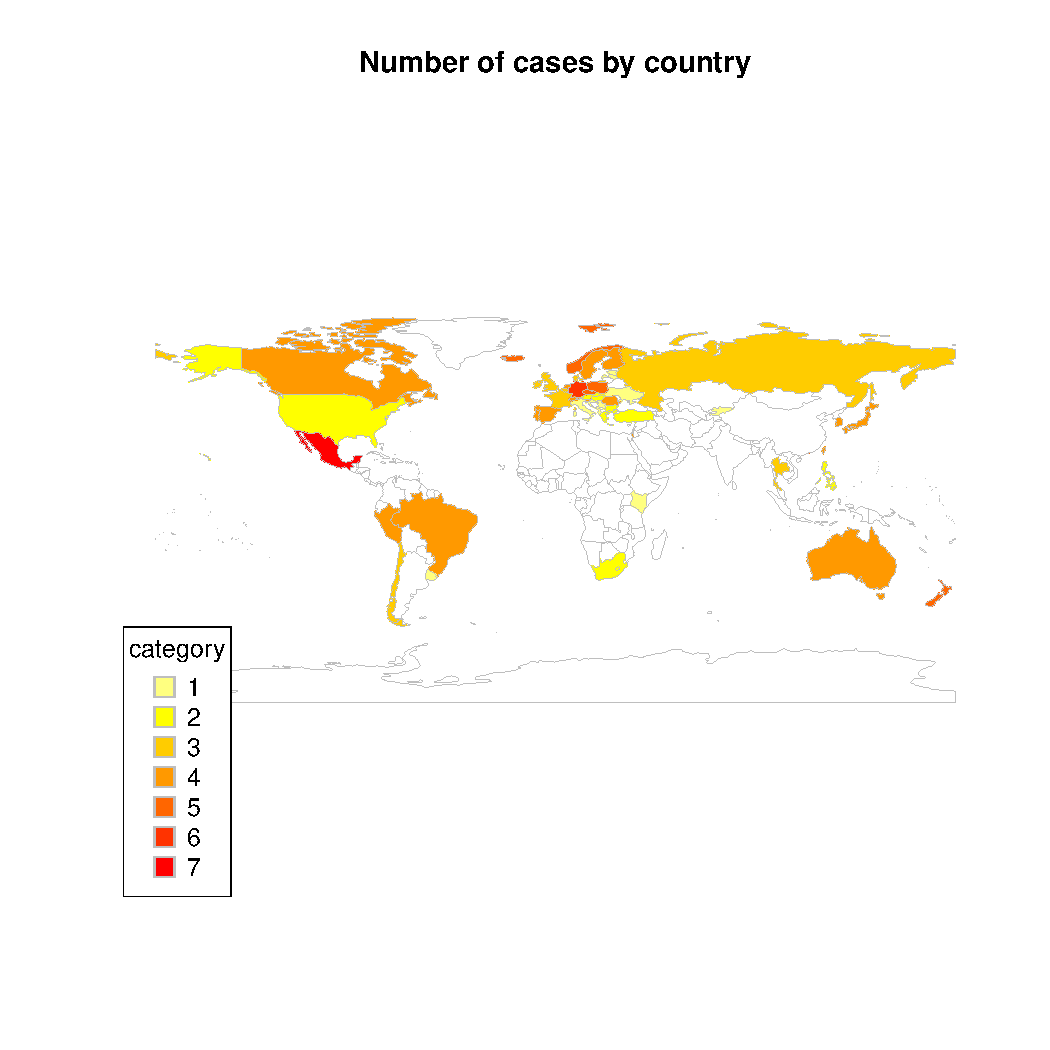
\includegraphics[width = .5 \textwidth]{../output/figures/case_map.pdf}
	\caption{Cases in CSES data, by country}
	\label{fig:case_map}
\end{figure}

The mean number of respondents in each case is 1384 (with a standard deviation of 539). The 160 different surveys come from xx different countries from the time between 1996 and 2016. Figure~\ref{fig:map} maps the number of surveys in each country. (Do we need to say any more? Perhaps something about mean / sd of preference intensity and $\tau$?)

\subsection{Distribution of preferences} 

How different are the CSES cases from one another? Aside from the intensity of preferences, we can describe each case with the vector $\bf \tilde{v}$, where the three-item vector $(v_1 + v_2, v_3 + v_4, v_5 + v_6)$ describes the distribution of first preferences, and the three-item vector $(m_{AB} = \frac{v_1}{v_1 + v_2}, m_{BA} = \frac{v_3}{v_3 + v_4}, m_{CB} = \frac{v_6}{v_5 + v_6})$ describes the distribution of second preferences. 

To link these two distributions together and classify cases more completely, we offer the following approach. Without loss of generality, let the candidate (party) $X$ whose first-preference voters have the most equally split second preferences, and the other two parties $Y$ and $Z$. If both $m_{YZ}$, $m_{ZY} > 0.6$, then classify this case as \emph{single-peaked} and denote it $X+$.\footnote{$X$ is the attractor: both remaining parties have a majority of their second preferences tilted towards $X$.} Conversely, if both $m_{YZ}, m{ZY} < 0.4$, then classify this case as \emph{divided majority} and denote it $X-$.\footnote{Here, $X$ is the repeller: both remaining parties have a majority of their second preferences tilted towards each other and away from $X$.} If $m_{YZ}, m_{ZY} \in [0.4, 0.6]$, then classify this case as \emph{neutral} and denote it $N(X)$. If neither of these conditions hold (because of unusual second preferences), classify it as \emph{other} and denote it $O$. This completes a mutually exclusive and exhaustive set of classes determined by $\bf \tilde{v}$.

\begin{table}[tb]
	\caption{Distribution of preference profiles in CSES data}
	\label{tab:csesprefs}
	\centering

	\begin{tabular}{lccc}
	\hline

	\toprule
	\textbf{} & \textbf{A} & \textbf{B} & \textbf{C} \\
	\cmidrule{2-4}
	Single-peaked (+) & 18 & 23 & 9  \\
	Divided majority (-) & 28 & 20 & 20  \\
	Neutral () & 5 & 7 & 3  \\
	Other () & & 27 &  \\
	\bottomrule
	\end{tabular}
\end{table}

Table~\ref{tab:csesprefs} summarises the distribution of preference classes across the CSES cases. A plurality of cases belong to the divided majority classes; however, there is also a large number of single-peaked cases, whereas neutral and others tend to be rarer. (Figure~\ref{fig:cses_fp} plots the distribution of first preferences conditional on the classes.)

\begin{figure}[!htb]
	\centering
	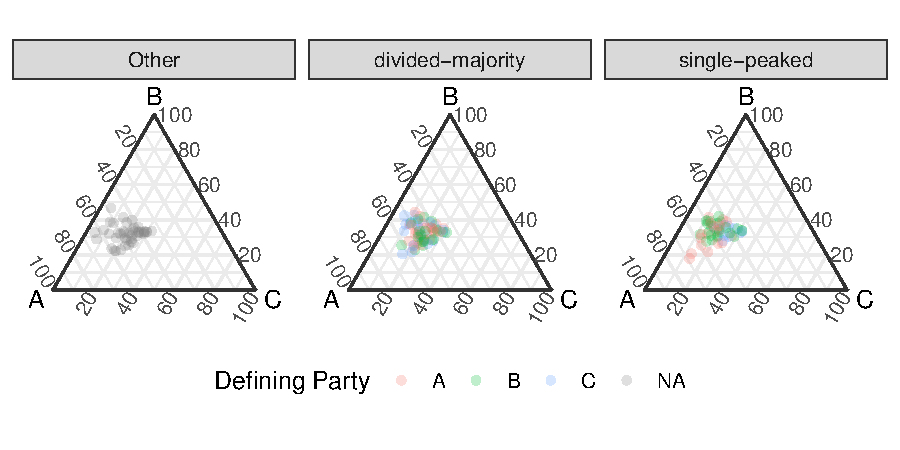
\includegraphics[width = 0.6 \textwidth]{../output/figures/cses_fp.pdf}
	\caption{Distribution of first preferences in CSES cases, by class}
	\label{fig:cses_fp}
\end{figure}

\section{Results}

Section 2 describes our analytical approach, which we apply to the CSES data described in Section 4. For each case in the CSES, we obtain a matrix $\bf X$, where the rows correspond to respondents, and each row $x_i\trans = [\tau_{Ii}, \tau_{Pi}]$.\footnote{Shorthand notation: $\tau_{I}$ is the strategic incentive under \textbf{I}RV, and $\tau_{P}$ is the strategic incentive under \textbf{P}lurality.} In this section, we present our main results.

\subsection{Convergence}

\begin{figure}[]
	\centering
	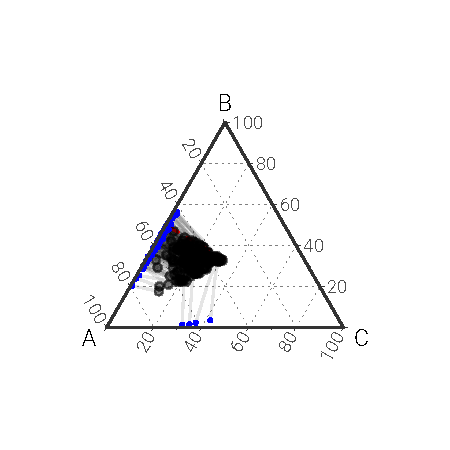
\includegraphics[width = .4\textwidth]{../output/figures/tatonnement_plur}
	\caption{Distribution of ballot shares in iterative process.}
	\label{}
\end{figure}

\begin{figure}[]
	\centering
	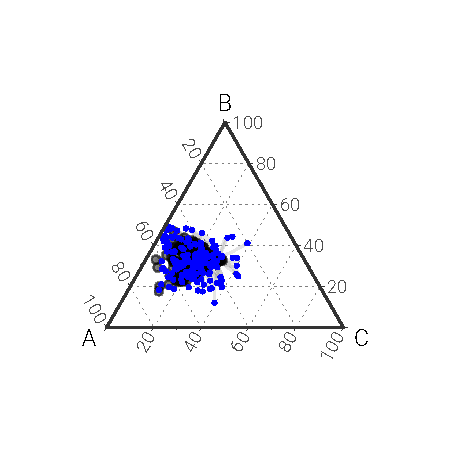
\includegraphics[width = .4\textwidth]{../output/figures/tatonnement_rcv}
	\caption{Distribution of ballot shares in iterative process.}
	\label{}
\end{figure}

\begin{figure}[]
	\centering
	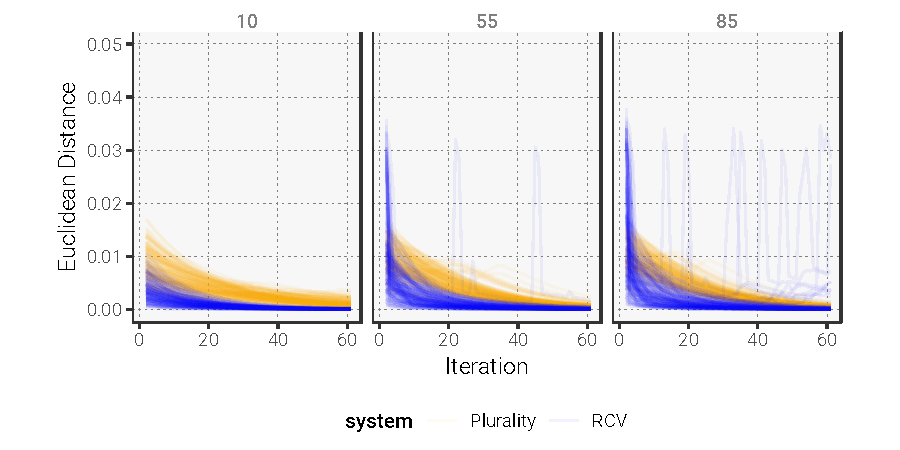
\includegraphics[width = .7\textwidth]{../output/figures/euclidean}
	\caption{Distribution of ballot shares in iterative process.}
	\label{}
\end{figure}

\subsection{Strategic Incentives}

\begin{figure}[]
	\centering
	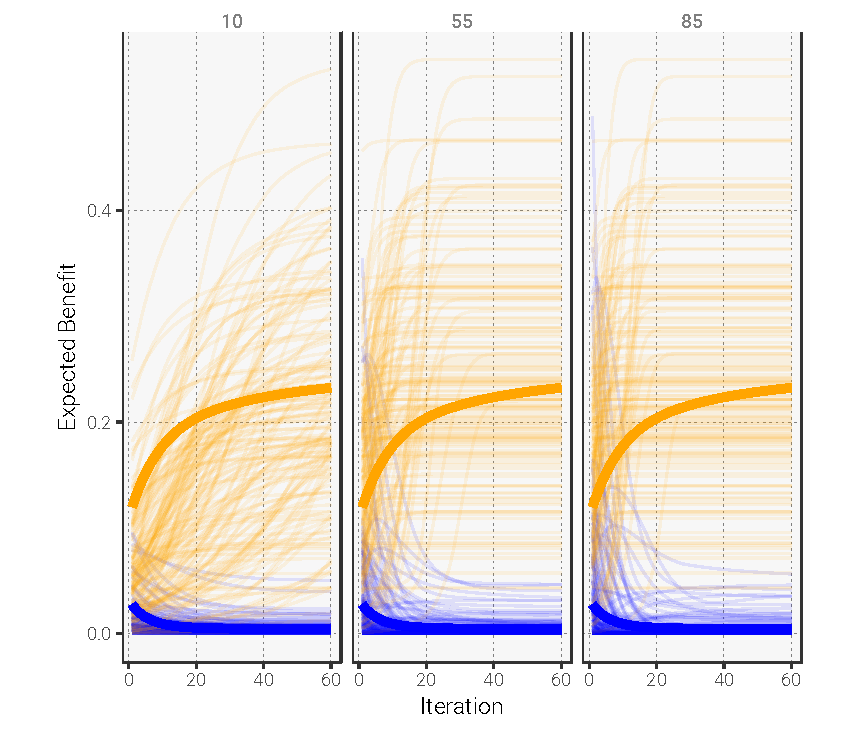
\includegraphics[width = .7\textwidth]{../output/figures/iterated_expbenefit}
	\caption{Distribution of ballot shares in iterative process.}
	\label{}
\end{figure}

\section{Conclusion}



\end{document}